% ----------------------------------------------------------------------------------------------------------------------
%       MPI PRACTISE
% ----------------------------------------------------------------------------------------------------------------------

\documentclass[onecolumn]{article}
\usepackage[utf8]{inputenc}   %con esto, voy a permitir los acentos sin menester del codigo
\usepackage[spanish]{babel}
%%%%%%%%%%%%%%%%%%%%%%%%%%%%%%%%%%%%%%%%%%%
\usepackage{graphicx,epsfig}
\usepackage{mathtools}
\usepackage{amsfonts,amsmath,amssymb,amsthm} 
\usepackage{relsize}
\usepackage{dcolumn}
\usepackage{array}
\usepackage{graphicx}
\usepackage{ulem}
\usepackage{subfig}
\usepackage{sidecap}
%\usepackage{wrapfig}
\usepackage{lipsum}
\usepackage{hyperref}
\usepackage{floatrow}
\usepackage{fancyhdr}
\usepackage{bm} %bold math symbols
\usepackage{hhline}

%%%%%%%%%%%%%%%%%%%%%%%%%%%%%%%%%%%%%%%%%%%
\newfloatcommand{capbtabbox}{table}[][\FBwidth]
\renewcommand{\vec}[1]{\mathbf{#1}} 
\renewcommand{\it}[1]{\textit{#1}}
\renewcommand{\d}{\text{d}}

\begin{document}

% --- Configurar la pagina ---------------------
\pagestyle{fancy}
\lhead{\bf EIA informe}
\rhead{Team}
%\lfoot{ }
\rfoot{Barcelona, March 2017}
% ----------------------------------------------


\title{EIA : Plantilla sencilla y cutre tipo artículo, una columna. Acentos disponibles.}
\author{Author: All of us}
\date{Wednesday, 29th March}

\maketitle

\section{Introduction}


\section{Initialisation of the system}

\section{Forces Elena}

\section{Forces Xabi}



\section{Euler Integrator}


\section{Verlet Integrator}


\section{PBC}


\section{Cálculo de magnitudes en equilibrio: Presión y temperatura}

 %\section{Cálculo de magnitudes en equilibrio: Presión y temperatura}

% %\section{Cálculo de magnitudes en equilibrio: Presión y temperatura}

% %\section{Cálculo de magnitudes en equilibrio: Presión y temperatura}

% \input{oscar}

\subsection{Presión y temperatura:}
Para el cálculo de la presión hemos hecho uso del teorema del virial que nos relaciona el promedio del trabajo de todas las partículas (la energía potencial) con la energía cinética promedia.

\begin{equation}
\left\langle E_c \right\rangle= -\frac{1}{2} \left\langle \vec{F}^{\text{TOT}} \circ \vec{r} \right\rangle
\label{eq:virial}
\end{equation}

Descomponemos la fuerza total como la suma de la fuerza interna debido a la interacción entre partículas y la externa al sistema:

\begin{equation}
\vec{F}^{\text{TOT}} = \vec{F}^{\text{int}}+\vec{F}^{\text{ext}}
\end{equation}

Es promedio del trabajo de las fuerzas externas será debido a la presión que ejerce la caja. Descomponiendo por componentes, dicha fuerza externa obtenemos la relación del promedio del trabajo externo con la presión:
\begin{equation}
\left\langle W^{ext}	\right\rangle = L_x (-PL_yL_z)+L_y (-PL_xL_z)+L_z (-PL_xL_y)= -3PV
\end{equation}

Donde $L_x$ es el valor del lado $x$ de la caja (ídem para $L_y$ y $L_z$).

Utilizando el teorema de equipartición de la energía:
\begin{equation}
\left\langle E_c \right\rangle= \frac{3}{2} N k_B T
\label{eq:particion}
\end{equation}

en la ecuación \ref{eq:virial}, obtenemos que la presión vale:
\begin{equation}
P = \frac{Nk_BT}{V}+\frac{1}{3}\left\langle \vec{F}^{\text{int}} \circ \vec{r} \right\rangle
\label{eq:presion}
\end{equation}

Para la temperatura hemos usado el teorema de equipartición de la energía (eq. \ref{eq:particion}):
\begin{equation}
T = \frac{1}{3m} \left\langle \vec{v}^2 \right\rangle
\label{eq:temp}
\end{equation}

\subsection{Implementació:}
Viendo las expresiones \ref{eq:presion} y \ref{eq:temp}, podemos ver que por cada magnitud hay que hacer la suma de $N$ productos escalares y luego sumarles i/o multiplicar unas constantes. Así que la implementación del cálculo de ambas magnitudes son muy parecidas.

En términos de paralelización, lo que he hecho es hacer que cada procesador me coja el mismo número de partículas a excepción del último que me cogerá el resto que queden. Luego lo que hará cada procesador será la suma parcial de dichos productos escalares y luego con la subrutina \textsf{MPI\_REDUCE}

\subsection{Presión y temperatura:}
Para el cálculo de la presión hemos hecho uso del teorema del virial que nos relaciona el promedio del trabajo de todas las partículas (la energía potencial) con la energía cinética promedia.

\begin{equation}
\left\langle E_c \right\rangle= -\frac{1}{2} \left\langle \vec{F}^{\text{TOT}} \circ \vec{r} \right\rangle
\label{eq:virial}
\end{equation}

Descomponemos la fuerza total como la suma de la fuerza interna debido a la interacción entre partículas y la externa al sistema:

\begin{equation}
\vec{F}^{\text{TOT}} = \vec{F}^{\text{int}}+\vec{F}^{\text{ext}}
\end{equation}

Es promedio del trabajo de las fuerzas externas será debido a la presión que ejerce la caja. Descomponiendo por componentes, dicha fuerza externa obtenemos la relación del promedio del trabajo externo con la presión:
\begin{equation}
\left\langle W^{ext}	\right\rangle = L_x (-PL_yL_z)+L_y (-PL_xL_z)+L_z (-PL_xL_y)= -3PV
\end{equation}

Donde $L_x$ es el valor del lado $x$ de la caja (ídem para $L_y$ y $L_z$).

Utilizando el teorema de equipartición de la energía:
\begin{equation}
\left\langle E_c \right\rangle= \frac{3}{2} N k_B T
\label{eq:particion}
\end{equation}

en la ecuación \ref{eq:virial}, obtenemos que la presión vale:
\begin{equation}
P = \frac{Nk_BT}{V}+\frac{1}{3}\left\langle \vec{F}^{\text{int}} \circ \vec{r} \right\rangle
\label{eq:presion}
\end{equation}

Para la temperatura hemos usado el teorema de equipartición de la energía (eq. \ref{eq:particion}):
\begin{equation}
T = \frac{1}{3m} \left\langle \vec{v}^2 \right\rangle
\label{eq:temp}
\end{equation}

\subsection{Implementació:}
Viendo las expresiones \ref{eq:presion} y \ref{eq:temp}, podemos ver que por cada magnitud hay que hacer la suma de $N$ productos escalares y luego sumarles i/o multiplicar unas constantes. Así que la implementación del cálculo de ambas magnitudes son muy parecidas.

En términos de paralelización, lo que he hecho es hacer que cada procesador me coja el mismo número de partículas a excepción del último que me cogerá el resto que queden. Luego lo que hará cada procesador será la suma parcial de dichos productos escalares y luego con la subrutina \textsf{MPI\_REDUCE}

\subsection{Presión y temperatura:}
Para el cálculo de la presión hemos hecho uso del teorema del virial que nos relaciona el promedio del trabajo de todas las partículas (la energía potencial) con la energía cinética promedia.

\begin{equation}
\left\langle E_c \right\rangle= -\frac{1}{2} \left\langle \vec{F}^{\text{TOT}} \circ \vec{r} \right\rangle
\label{eq:virial}
\end{equation}

Descomponemos la fuerza total como la suma de la fuerza interna debido a la interacción entre partículas y la externa al sistema:

\begin{equation}
\vec{F}^{\text{TOT}} = \vec{F}^{\text{int}}+\vec{F}^{\text{ext}}
\end{equation}

Es promedio del trabajo de las fuerzas externas será debido a la presión que ejerce la caja. Descomponiendo por componentes, dicha fuerza externa obtenemos la relación del promedio del trabajo externo con la presión:
\begin{equation}
\left\langle W^{ext}	\right\rangle = L_x (-PL_yL_z)+L_y (-PL_xL_z)+L_z (-PL_xL_y)= -3PV
\end{equation}

Donde $L_x$ es el valor del lado $x$ de la caja (ídem para $L_y$ y $L_z$).

Utilizando el teorema de equipartición de la energía:
\begin{equation}
\left\langle E_c \right\rangle= \frac{3}{2} N k_B T
\label{eq:particion}
\end{equation}

en la ecuación \ref{eq:virial}, obtenemos que la presión vale:
\begin{equation}
P = \frac{Nk_BT}{V}+\frac{1}{3}\left\langle \vec{F}^{\text{int}} \circ \vec{r} \right\rangle
\label{eq:presion}
\end{equation}

Para la temperatura hemos usado el teorema de equipartición de la energía (eq. \ref{eq:particion}):
\begin{equation}
T = \frac{1}{3m} \left\langle \vec{v}^2 \right\rangle
\label{eq:temp}
\end{equation}

\subsection{Implementació:}
Viendo las expresiones \ref{eq:presion} y \ref{eq:temp}, podemos ver que por cada magnitud hay que hacer la suma de $N$ productos escalares y luego sumarles i/o multiplicar unas constantes. Así que la implementación del cálculo de ambas magnitudes son muy parecidas.

En términos de paralelización, lo que he hecho es hacer que cada procesador me coja el mismo número de partículas a excepción del último que me cogerá el resto que queden. Luego lo que hará cada procesador será la suma parcial de dichos productos escalares y luego con la subrutina \textsf{MPI\_REDUCE}

\section{Visual}

A continuación se detallará el procedimiento seguido en la implementación de la paralelización del código de análisis visual, última parte del código de dinámica molecular desarrollado.

Para esta parte se decide calcular el desplazamiento cuadrático medio (MSD) de las partículas a lo largo de la simulación, con la expresión:
\begin{equation}\label{eq: expresion msd alberto}
MSD \equiv \langle\left(x(t)-x_{o}\right)^{2}\rangle
\end{equation}

Para calcular dicha expresión, se introduce en el archivo de entrada un valor de la frecuencia de escritura de las posiciones de las partículas (\it{restart}) y en el  \it{main} del archivo que las contiene (con el mismo nombre y extensión \it{rst}). Del mismo modo, al iniciar la simulación se determina el número de frames que contendrá el archivo de restart.

Una vez finalizada la simulación, previamente a finalizar el entorno MPI, se llama a la subrutina \it{postvisual} con la entrada de número de frames, número de partículas y dimensión del sistema.

La subrutina (en serie y en paralelo) lee el archivo generado a lo largo de la dinámica molecular en una matriz. Posteriormente, mide para cada partícula el MSD a cada frame impreso. Es decir, para una misma partícula conociendo el número de frames y partículas del sistema recorre la matriz calculando la expresión \ref{eq: expresion msd alberto}. Dichos valores se van imprimiendo en una nueva matriz con F filas (correspondientes una a cada tiempo) y C columnas (una por cada partícula).

Finalmente, el resultado se imprime en un archivo con nombre \it{desplazamientos.dat}.

\subsection{Implementación en paralelo}
Se decide que la paralelización de la rutina se realice dividiendo las N partículas del sistema en los diferentes procesadores a usar. De este modo, se consigue que cada procesador pueda calcular el valor de MSD con la rutina ya generada para las partículas asignadas de manera autónoma, y sólo deba comunicarse con los demás al finalizar el cálculo.

Por otra parte, la lectura del archivo \it{restart.rst} se realiza también en paralelo. Éste hecho se debe a que en un primer momento se realizaba de manera única a través del MASTER y éste enviaba a cada procesador el rango correspondiente --según la división de partículas realizada-- de la matriz de entrada para que realizara el cálculo. Se observaron problemas de comunicación por parte del MASTER a los procesadores y se decidió implementar también la lectura en paralelo.

Con la lectura en paralelo se han observado los siguientes resultados:
\begin{itemize}
\item Desaparición de los problemas de comunicación existentes, al no tener que comunicarse el MASTER con cada procesador.
\item Tiempo de cálculo similar en ambos métodos, ya que la lectura del archivo se debía realizar de todos modos.
\end{itemize}
Se debe considerar que pese a que el tiempo de cálculo no aumenta, el gasto de memoria sí que incrementa debido a que la lectura del archivo \it{restart.rst} es realizada por todos los procesadores. En cualquier caso, se hace un balance positivo ya que en el método anterior intentado se habían producido problemas en algunos tests realizados a nivel de comunicación que no se habían podido solucionar.

Posteriormente, cada procesador calcula el MSD para las partículas asignadas en la división de trabajo realizada y mandan los rangos de la matriz de desplazamientos a MASTER. Éste, después de recibir los datos, los imprime en el archivo de resultados final.

Así, el proceso se puede resumir como:
\begin{enumerate}
\item Lectura del archivo de entrada completo en paralelo.
\item Cálculo del MSD en paralelo, con división por partículas en los diferentes procesadores.
\item Envío de valores de MSD de los diferentes procesadores a MASTER.
\item Impresión de los resultados en \it{desplazamientos.dat}.
\end{enumerate}

\subsection{Análisis de la implementación en paralelo}
La implementación en paralelo se ha realizado de manera satisfactoria obteniendo unos resultados de disiminución de tiempo considerables en aumentar el número de procesadores.

Para diferente número de partículas (figura \ref{fig: comparacion cores alberto} se ha analizado el tiempo de cálculo de la rutina para un número creciente de procesadores (de 1 --en serie-- a 12) observando como la disminución del tiempo de cálculo es considerable entre 2 y 6 procesadores, pero a partir de éstos el tiempo es muy parecido.
\begin{figure}
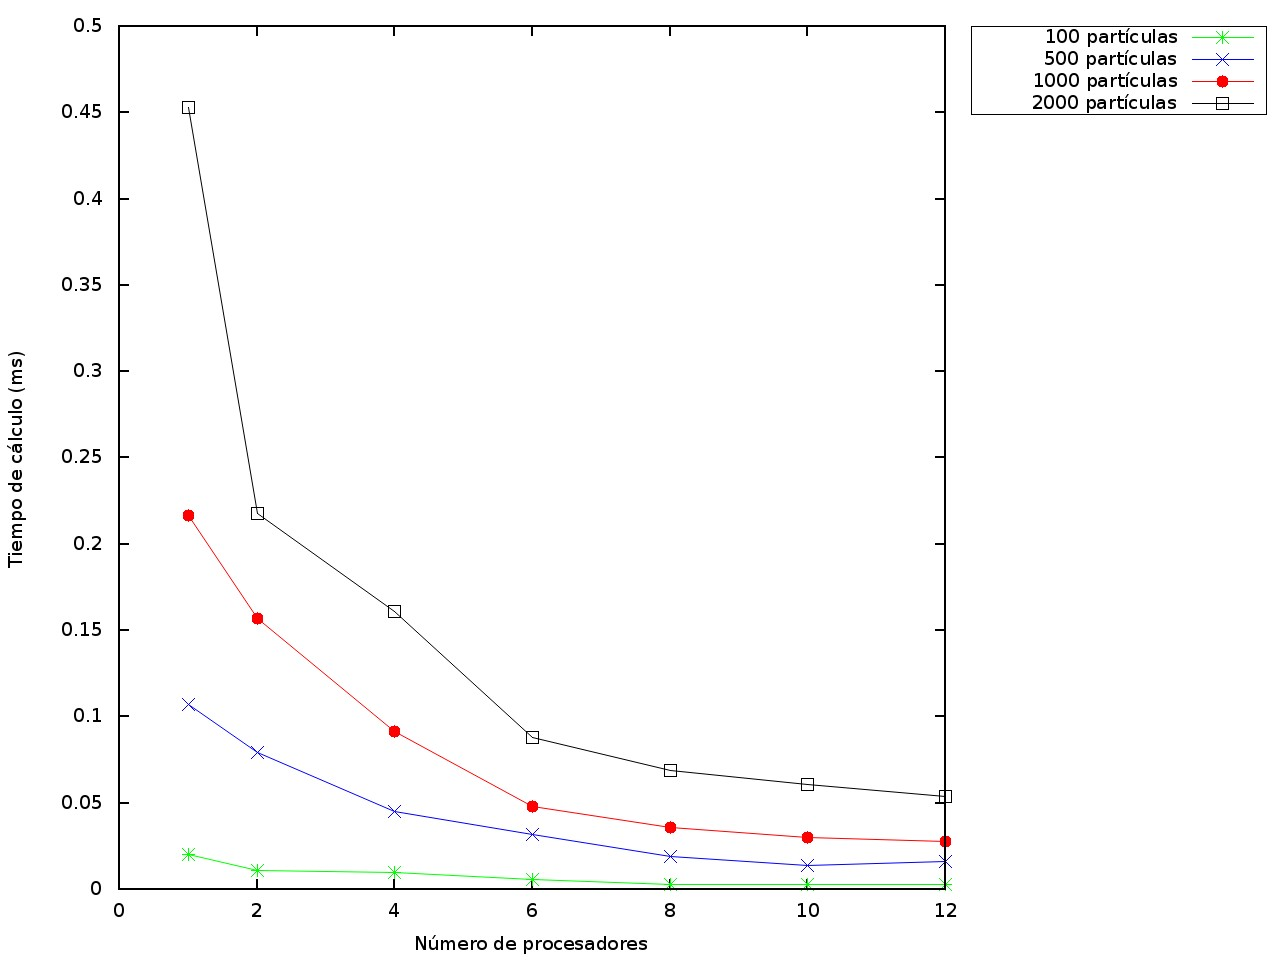
\includegraphics[scale=0.25]{velos_calc_alberto.jpeg} 
\caption{Tiempo de cálculo (ms) para diferentes sistemas (N=100,\ 500,\ 1000,\ 2000) en función de los procesadores utilizados.} 
\label{fig: comparacion cores alberto}
\end{figure}

Se puede observar como para sistemas de mayor tamaño (N=1000,2000) la disminución de velocidad entre el cálculo en serie y con dos procesadores es remarcable. Prácticamente, con 2000 partículas en aumentar el número de procesadores en dos se consiguen tiempos de cálculo comparables al sistema de 1000 partículas con dos procesadores menos. A partir de 8 procesadores dicha tendencia se pierde obteniendo un comportamiento asintótico.

Analizando el tiempo de cálculo para el mismo número de procesadores en aumentar el de partículas obtenemos un incremento lineal del tiempo, tal y como se puede observar en la figura \ref{fig: comparacionparticulasalberto}.
\begin{figure}[h!]
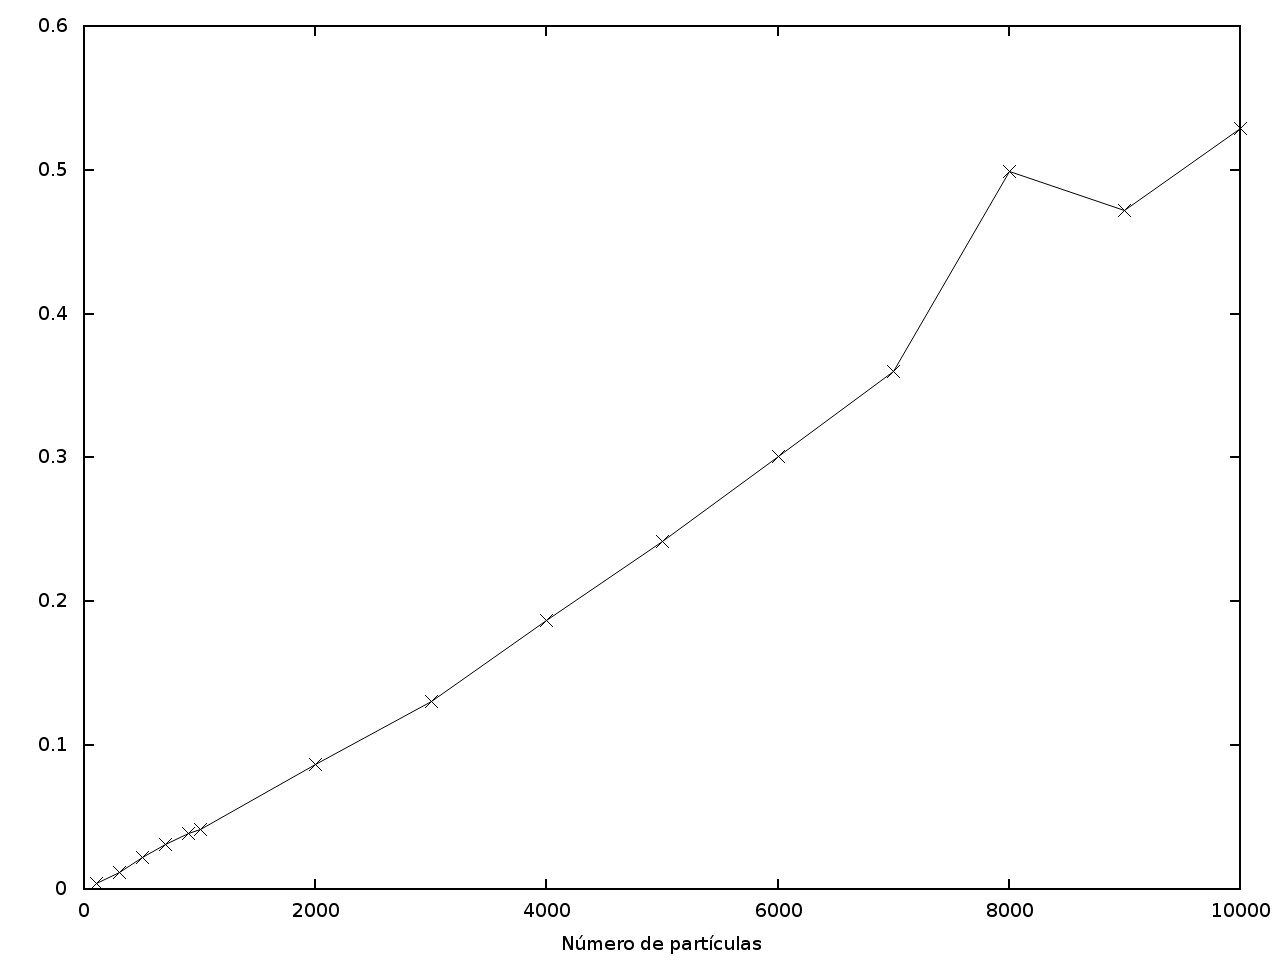
\includegraphics[scale=0.25]{8_cores_alberto.jpeg} 
\caption{Tiempo de cálculo (ms) para seis procesadores en función del tamaño del sistema.} 
\label{fig: comparacionparticulasalberto}
\end{figure}
En este caso, se puede observar una dependencia cuasi-lineal respecto el tiempo de cálculo y el tamaño del sistema.

\subsection{Conclusiones}
Del proceso de paralelización de la rutina de cálculo del desplazamiento cuadrático medio de las partículas, podemos concluir:
\begin{itemize}
\item El proceso de paralelización a través de la división por partículas permite disminuir el tiempo de cálculo de manera relevante en aumentar los procesadores utilizados, equiparando la velocidad a sistemas más pequeños para un número de procesadores menor o igual a 6.
\item Dicha disminución del tiempo de cálculo no se observa para un número de procesadores mayor a 6, ya que se observa un comportamiento asintótico.
\item Para un mismo número de procesadores, hay una relación cuasi-lineal entre el tiempo de cálculo y el tamaño del sistema.
\item La paralelización, pues, es efectiva para pocos procesadores y permite calcular sistemas 4 veces mayores en el mismo tiempo (veáse figura \ref{fig: comparacion cores alberto}, la velocidad para el sistema con 2000 partículas con 6 procesadores es similar al cálculo en serie con 500 partículas). 
\end{itemize}
\end{document}
